% -----------------------------------------------
% Template for ISMIR Papers
% 2016 version, based on previous ISMIR templates

% Requirements :
% * 6+1 page length maximum
% * 2MB maximum file size
% * Copyright note must appear in the bottom left corner of first page
% (see conference website for additional details)
% -----------------------------------------------

\documentclass{article}
\usepackage{ismir,amsmath,cite}
\usepackage{graphicx}
\usepackage{color}
\usepackage[]{units}
\usepackage{microtype}

% Title.
% ------
\title{On drum playing technique detection in polyphonic mixtures}

% Note: Please do NOT use \thanks or a \footnote in any of the author markup

% Single address
% To use with only one author or several with the same address
% ---------------
%\oneauthor
% {Names should be omitted for double-blind reviewing}
% {Affiliations should be omitted for double-blind reviewing}

% Two addresses
% --------------
%\twoauthors
%  {Chih-Wei Wu} {Georgia Institute of Technology \\ Center for Music Technology}
%  {Alexander Lerch} {\{cwu307, alexander.lerch\}@gatech.edu}

%% To make customize author list in Creative Common license, uncomment and customize the next line
%  \def\authorname{First Author, Second Author} 


% Three addresses
% --------------
\threeauthors
  {First Author} {Affiliation1 \\ {\tt author1@ismir.edu}}
  {Second Author} {\bf Retain these fake authors in\\\bf submission to preserve the formatting}
  {Third Author} {Affiliation3 \\ {\tt author3@ismir.edu}}

%% To make customize author list in Creative Common license, uncomment and customize the next line
%  \def\authorname{First Author, Second Author, Third Author} 

% Four or more addresses
% OR alternative format for large number of co-authors
% ------------
%\multauthor
%{First author$^1$ \hspace{1cm} Second author$^1$ \hspace{1cm} Third author$^2$} { \bfseries{Fourth author$^3$ \hspace{1cm} Fifth author$^2$ \hspace{1cm} Sixth author$^1$}\\
%  $^1$ Department of Computer Science, University , Country\\
%$^2$ International Laboratories, City, Country\\
%$^3$  Company, Address\\
%{\tt\small CorrespondenceAuthor@ismir.edu, PossibleOtherAuthor@ismir.edu}
%}
%\def\authorname{First author, Second author, Third author, Fourth author, Fifth author, Sixth author}


\sloppy % please retain sloppy command for improved formatting

\begin{document}

%
\maketitle
%
\begin{abstract}
%In this paper, the problem of drum playing technique detection in the polyphonic mixtures of music is addressed, and a system using features extracted from the Non-negative Matrix Factorization (NMF) activation functions is presented. The proposed method focuses on detecting 4 rudimentary techniques: \textit{strike}, \textit{buzz roll}, \textit{flam} and \textit{drag}. To evaluate the system, two datasets are introduced for both training and testing purposes. For training, a dataset consisting of the 4 major rudiments has been created. For testing, the ENST drum dataset minus one subset has been manually annotated. The evaluation process includes a comparison of different sets of features under different controlled conditions. In this preliminary work towards drum playing technique detection in the real-world recordings, we show the capability of the proposed system as well as the challenges and limitations in the context of polyphonic mixtures. The results demonstrate the potential of using NMF activation functions to obtain more detailed information about the drum playing, however, the performance in the polyphonic mixtures has to be improved with further investigations on different pre-processing steps in the future. 

In this paper, the problem of drum playing technique detection in polyphonic mixtures of music is addressed. We focus on the identification of 4 rudimentary techniques: strike, buzz roll, flam, and drag. The specifics and the challenges of this task are being discussed, and different sets of features are compared, including baseline spectral features, as well as various features extracted from NMF-based activation functions. We investigate the capabilities and limitations of
the presented system in the case of real-world recordings and polyphonic mixtures. To design and evaluate the system, two datasets are introduced: a
training dataset generated from individual drum hits, and additional annotations of the well-known ENST drum dataset minus one subset as test dataset. The results demonstrate issues with the traditionally used spectral features, and indicate the potential of using NMF activation functions for playing technique detection, however, the performance of polyphonic music still leaves room for future improvement.
\end{abstract}

%
% what's the key ideas in this paper?
% 1. previous publications only focus classifying the one-shot samples of different playing sounds, in this paper we focus on detecting the playing techniques in 
%     the real recordings of polyphonic mixtures
% 2. we show that the timbral features, despite their efficiency in distinquishing different sounds, might not be feasible for classifying different techniques
%     especially for techinques consisting of multiple drum strokes
% 3. we also show that the activation-based features worked when the events are perfectly segmented. This shows that the activation function actually contains 
%     the information for distinquishing these techniques
% 4. although the accuracy of the current system in the polyphonic mixtures is still low, it demonstrates the potential of using activation-based features
%     for transcribing subtle gestures from the audio signals.
% 5. future work: pre-processing steps for source separation, better segmentation schemes, and test other classifiers

\section{Introduction}\label{sec:introduction}

Automatic Music Transcription (AMT), one of the most popular research topics in the Music Information Retrieval (MIR) community, is the process of transcribing the musical events in the audio signal into a notation such as MIDI or sheet music. In spite of being intensively studied, there still remain many unsolved problems and challenges in AMT \cite{Benetos2013}. One of the challenges is the extraction of additional information, such as dynamics, expressive notation and articulation, in order to produce a more complete description of the music performance. 

For pitched instruments, most of the work in AMT mainly focuses on tasks such as melody extraction \cite{Bittner2015a}, chord estimation \cite{Humphrey2015}, and instrument recognition \cite{Hamel2009}. Few studies try to expand the scope to playing technique and expression detection for instruments such as electric guitar \cite{Su2014a, Chen2015} and violin \cite{Li2015a}. Similarly, the main focus of AMT systems for percussive instruments has been put on recognizing the instrument types (e.g., HiHat (HH), Snare Drum (SD), Bass Drum (BD)) and their corresponding onset times \cite{Benetos2014, Dittmar2014, Thompson2014, Roebel2015, Wu2015a}. Studies on retrieving the playing techniques and expressions are relatively sparse. 

Since playing technique is an important layer of a musical performance for its deep connection to the timbre and subtle expressions of an instrument, an automatic system that transcribes such techniques may provide insights into the performance and facilitate other research in MIR. In this paper, we present a system that aims to detect the drum playing techniques within polyphonic mixtures of music. 
The contributions of this paper can be summarized as follows: first, to the best of our knowledge, this is the first study to investigate the automatic detection of drum playing techniques in polyphonic mixtures of music. The results may support the future development of a complete drum transcription system. Second, a comparison between the commonly used timbre features and features based on activation functions of a Non-Negative Matrix Factorization (NMF) system are presented and discussed. The results reveal problems with using common timbre features. Third, two datasets for training and testing are introduced. The release of these datasets is intended to encourage future research in this field. The data may also be seen as a core compilation to be extended in the future.

The remainder of the paper is structured as follows: in Sect.~\ref{sec:related_work}, related work in drum playing technique detection is introduced. The details of the proposed system and the extracted features are described in Sect.~\ref{sec:method}, and the evaluation process, metrics, and the experiment results are shown in Sect.~\ref{sec:eval}. Finally, the conclusion and future research directions are addressed in Sect.~\ref{sec:conclusion}. 

% summarize the contributions
% 1. training and testing dataset
% 2. comparison between commonly used audio features and activation-based features 
% 3. to the best of our knowledge, this paper is the first study to attempt the playing technique detection problem in the context of polyphonic mixtures

%
\section{Related work}\label{sec:related_work}
% what is playing technique for drums 
Percussive instruments, generating sounds through vibrations induced by strikes and other excitations, belong to the oldest musical instruments \cite{Rossing2001}. While the basic gesture is generally simple, the generated sounds can be complex depending on where and how the instrument is being excited. In western popular music, a drum set, which contains multiple instruments such as SD, BD, HH, etc., is one of the most commonly used percussion instruments. In general, every instrument in a drum set is excited using drum sticks. With good control of the drum sticks, variations in timbre can be created through different excitation methods and gestures\cite{Stone2009}. These gestures, sometimes referred to as rudiments, are the foundations of many drum playing techniques. These rudiments can be categorized into four types:\footnote{http://vicfirth.com/40-essential-rudiments/ Last Access: 2016/3/16}

\begin{table*}[]
\footnotesize
\centering
\begin{tabular}{llll}
\hline
\textbf{Dataset}                                                                                   & \textbf{Annotated Techniques}                                 & \textbf{Description}                                                                                                                      & \textbf{Total} \\ \hline
\multicolumn{1}{l|}{Data in {[}15{]}}                                                              & \multicolumn{1}{l|}{Strike, Rim Shot, Brush}                  & \multicolumn{1}{l|}{\begin{tabular}[c]{@{}l@{}}1 drum (snare), \\ 5 strike positions (from center to edge)\end{tabular}}                  & 1264 clips     \\ \hline
\multicolumn{1}{l|}{MDLib2.2 {[}16{]}}                                                             & \multicolumn{1}{l|}{Strike, Rim Shot, Buzz Roll, Cross Stick} & \multicolumn{1}{l|}{\begin{tabular}[c]{@{}l@{}}9 drums, \\ 4 stick heights, \\ 3 stroke intensities, \\ 3 strike positions\end{tabular}}  & 10624 clips    \\ \hline
\multicolumn{1}{l|}{IDMT-Drum {[}9{]}}                                                             & \multicolumn{1}{l|}{Strike}                                   & \multicolumn{1}{l|}{\begin{tabular}[c]{@{}l@{}}3 drums (snare, bass and hihat), \\ 3 drum kits (real, waveDrum, technoDrum)\end{tabular}} & 560 clips      \\ \hline
\multicolumn{1}{l|}{\begin{tabular}[c]{@{}l@{}}ENST Drum \\ Minus One Subset {[}18{]}\end{tabular}} & \multicolumn{1}{l|}{Strike, Rim Shot, Brush, Cross Stick}     & \multicolumn{1}{l|}{\begin{tabular}[c]{@{}l@{}}13 drums, \\ 3 drum kits played by 3 drummers\end{tabular}}                                & 64 tracks      \\ \hline
\end{tabular}
\caption{An overview of publicly available datasets for drum transcription tasks}
\label{tab:data_all}
\end{table*}

\begin{enumerate}
	\item \textbf{Roll Rudiments}: drum rolls created by single or multiple bounce strokes (Buzz Roll).
	\item \textbf{Paradiddle Rudiments}: a mixture of alternative single and double strokes. 
	\item \textbf{Flam Rudiments}: drum hits with one preceding grace note.
	\item \textbf{Drag Rudiments}: drum hits with two preceding grace notes created by double stroke.
\end{enumerate}

There are also other playing techniques that are commonly used to create timbral variations in a drum set, such as \textit{Brush}, \textit{Cross Stick}, \textit{Rim Shot}, etc. Most drum transcription systems, however, focus on single strikes instead of these playing techniques \cite{Benetos2014, Dittmar2014, Thompson2014, Roebel2015, Wu2015a}. 

% 2004 paper
In an early attempt to retrieve percussion gestures from the audio signal, Tindale et al.~investigated the timbral variations of the snare drum sounds induced by different excitations \cite{Tindale2004}. Three expert players were asked to play on different locations on the snare drums (center, halfway, edge, etc.) with different excitation (strike, rim shot, and brush), resulting in a dataset with 1260 individual samples. The classification results for this dataset based on standard spectral and temporal features (e.g., centroid, flux, MFCCs, etc.) and classifiers (e.g., kNN and SVM) were reported, and an overall accuracy of around 90\% was achieved. Since the dataset is relatively small, howver, it is difficult to generalize the results to different scenarios.  

% 2013 paper
Following the same direction, Prockup et al. further explored the discrepancy between more expressive gestures with a larger dataset that covers multiple drums of a standard drum set \cite{Prockup2013}. A dataset was created with combinations of different drums, stick heights, stroke intensities, strike positions and articulations. Using a machine learning based approach similar to \cite{Tindale2004}, various features were extracted from the samples, and a Support Vector Machine (SVM) was trained to classify the sounds. An accuracy of over 95\% was reported on multiple drums with a 4-class SVM and features such as MFCCs, Spectral features, and the proposed evolution features. Both of the above mentioned studies showed promising results in the static classification, however, they were not evaluated with real-world drum recordings, and the applicability of these approaches for transcribing real-world drum recordings still needs to be tested. Additionally, the potential impact of polyphonic background music could be another concern of these approaches. 
 
% 2011 paper
Another way to retrieve more information from the drum performance is through the use of multi-modal data \cite{Hochenbaum2011}. Hochenbaum and Kapur investigated the inclusion of drum hand recognition in the data by capturing microphone and accelerometer data simultaneously. Two performers were asked to play the snare drum with four different rudiments (namely single stroke roll, double stroke open roll, single paradiddle and double paradiddle). Standard spectral and temporal features (e.g., centroid, skewness, zero-crossing rate, etc.) were extracted from the audio and accelerometer data, and different classifiers were applied and compared. With a Multi-Layer Perceptron (MLP), an accuracy of around 84\% was achieved for a 2-class drum hand classification task. It cannot be ruled out that the extra requirement of attaching the sensors on the performers' hands might alter the playing experience and thus deviate from the real playing gestures. Furthermore, this method does not allow the analysis of existing audio recordings. 

% A table for popular drum dataset, covered timbre. what did they miss in common? in this paper, what do we focus on?
In general, the above mentioned studies mainly focused on evaluating the discriminability of isolated samples. The evaluation on real-world drum recordings, i.e.\ recordings of a drummer continuously playing, is usually unavailable due to the lack of annotated datasets. In Table \ref{tab:data_all}, different datasets for drum transcription are presented. It can be found that most of the datasets only contain annotations of playing techniques that are easily distinguishable from the normal strike (e.g., Cross Stick, Brush, Rim Shot). For playing techniques such as Flam, Drag and Buzz Roll, there are no datasets and annotations available. 

%{\color{red}{the following is not related work. Find a better place}} Therefore, in this paper we focus on these missing parts, augment one existing dataset with corresponding annotations, investigate differences between these techniques, and attempt to transcribe them from real-world drum recordings under the influence of polyphonic music. The goal of this study is to enhance the existing drum transcription systems with more details on the drum performance, and facilitate research in music education, music style identification, and other related topics. 

% here I may emphasize the key ideas of this work and how it distinquishes itself from the others
% not just a static classification but actually apply to the real drum recordings

\begin{figure}
\centering
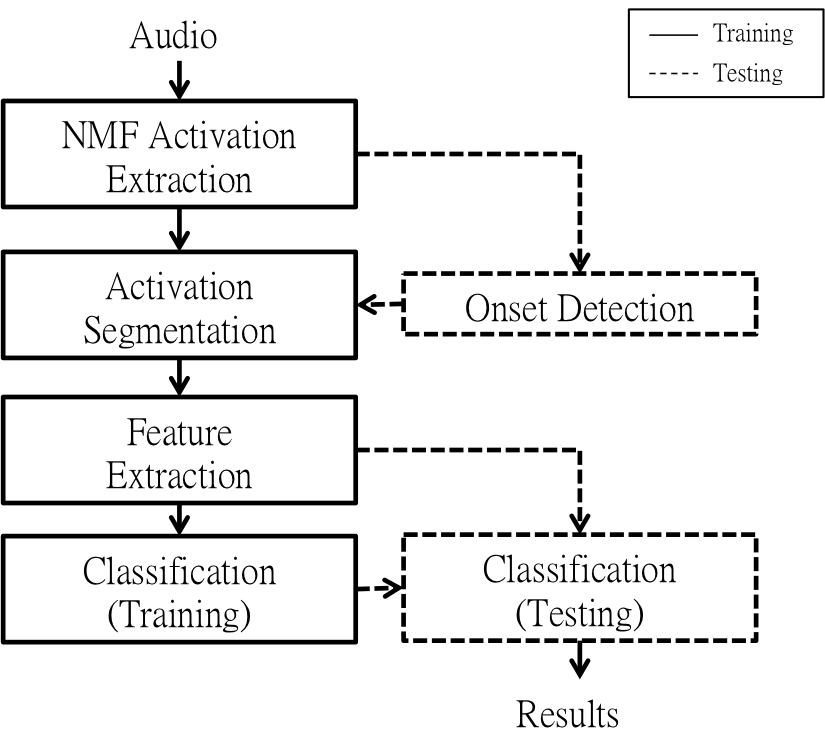
\includegraphics[width = 7 cm]{./figures/block_diagram.png}
\caption{Block diagram of the proposed system}
\label{fig:block}
\end{figure}

\section{Method}\label{sec:method}
\subsection{System Overview}\label{ssec:overview}

The block diagram of the proposed system is shown in Figure \ref{fig:block}. The system consists of two stages: training and testing. During the training stage, NMF activation functions (see Sect.~\ref{sssec:activ}) will first be extracted from the training data. Here, the training data only consists of audio clips with one-shot samples of different playing techniques. Next, features will be extracted from a short segment around the salient peak in the activation function (see Sect. \ref{sssec:activ}). Finally, all of the features and their corresponding labels will be used to train a classifier. The classes we focus on in this paper are: \{Strike, Roll, Drag, Flam\}. 

For the testing, a similar procedure is performed. When a longer drum recording is used as the testing data, an additional onset detection step is taken to narrow down the area of interest. %{\color{red} where to put this sentence?}
Since the focus of this paper is on playing technique detection, the onset detection step is bypassed by adopting the annotated ground truth in order to simulate the best case scenario. Once the features have been extracted from the segments, the pre-trained classifier can be used to classify the playing technique in the recordings. More details will be given in the following sections. 
 
\subsection{Feature Extraction}\label{ssec:featuresExtract}
\subsubsection{Activation Functions (AF)}
\label{sssec:activ}

To detect drum playing technique in polyphonic music, a transcription method that is robust against the influence of background music is required. In this paper, we applied the drum transcription scheme as described in \cite{Wu2015a} for its adaptability to polyphonic mixtures of music. The flowchart of the process is shown in Fig.~\ref{fig:nmf}. This method decomposes the magnitude spectrogram of the complex mixtures with a fixed pre-trained drum dictionary and a randomly initialized entries for harmonic contents. Once the signal is decomposed, the activation function $h_{i}(n)$ of each individual drum can be extracted, in which $n$ is the block index and $i = \{HH, SD, BD\}$ indicates the type of drum

All of the audio samples are mono with a sampling rate of \unit[44.1]{kHz}. The Short Time Fourier Transform (STFT) of is computed with a block size of 512 and a hop size of 128, and a Hann window is applied to each block. The harmonic rank $r_{h} $ for the partially-fixed NMF is  $50$, and the dictionary is trained from the ENST drum dataset \cite{Gillet2006}. The resulting $h_{i}(n)$ is scaled to a range between 0 and 1 and smoothed using a median filter with an order of $p = 5$ samples. Since a template in the dictionary is intended to capture the activity of the same type of drum, the drum sounds with slightly different timbres will still result in similar $h_{i}(n)$. Therefore, the extracted activation function $h_{i}(n)$ can be considered as a timbre invariant transformation and is desirable for detecting the underlying techniques. Segments of these activation functions can be used directly as features or as the intermediate representation for the extraction of other features. 

\begin{figure}
\centering
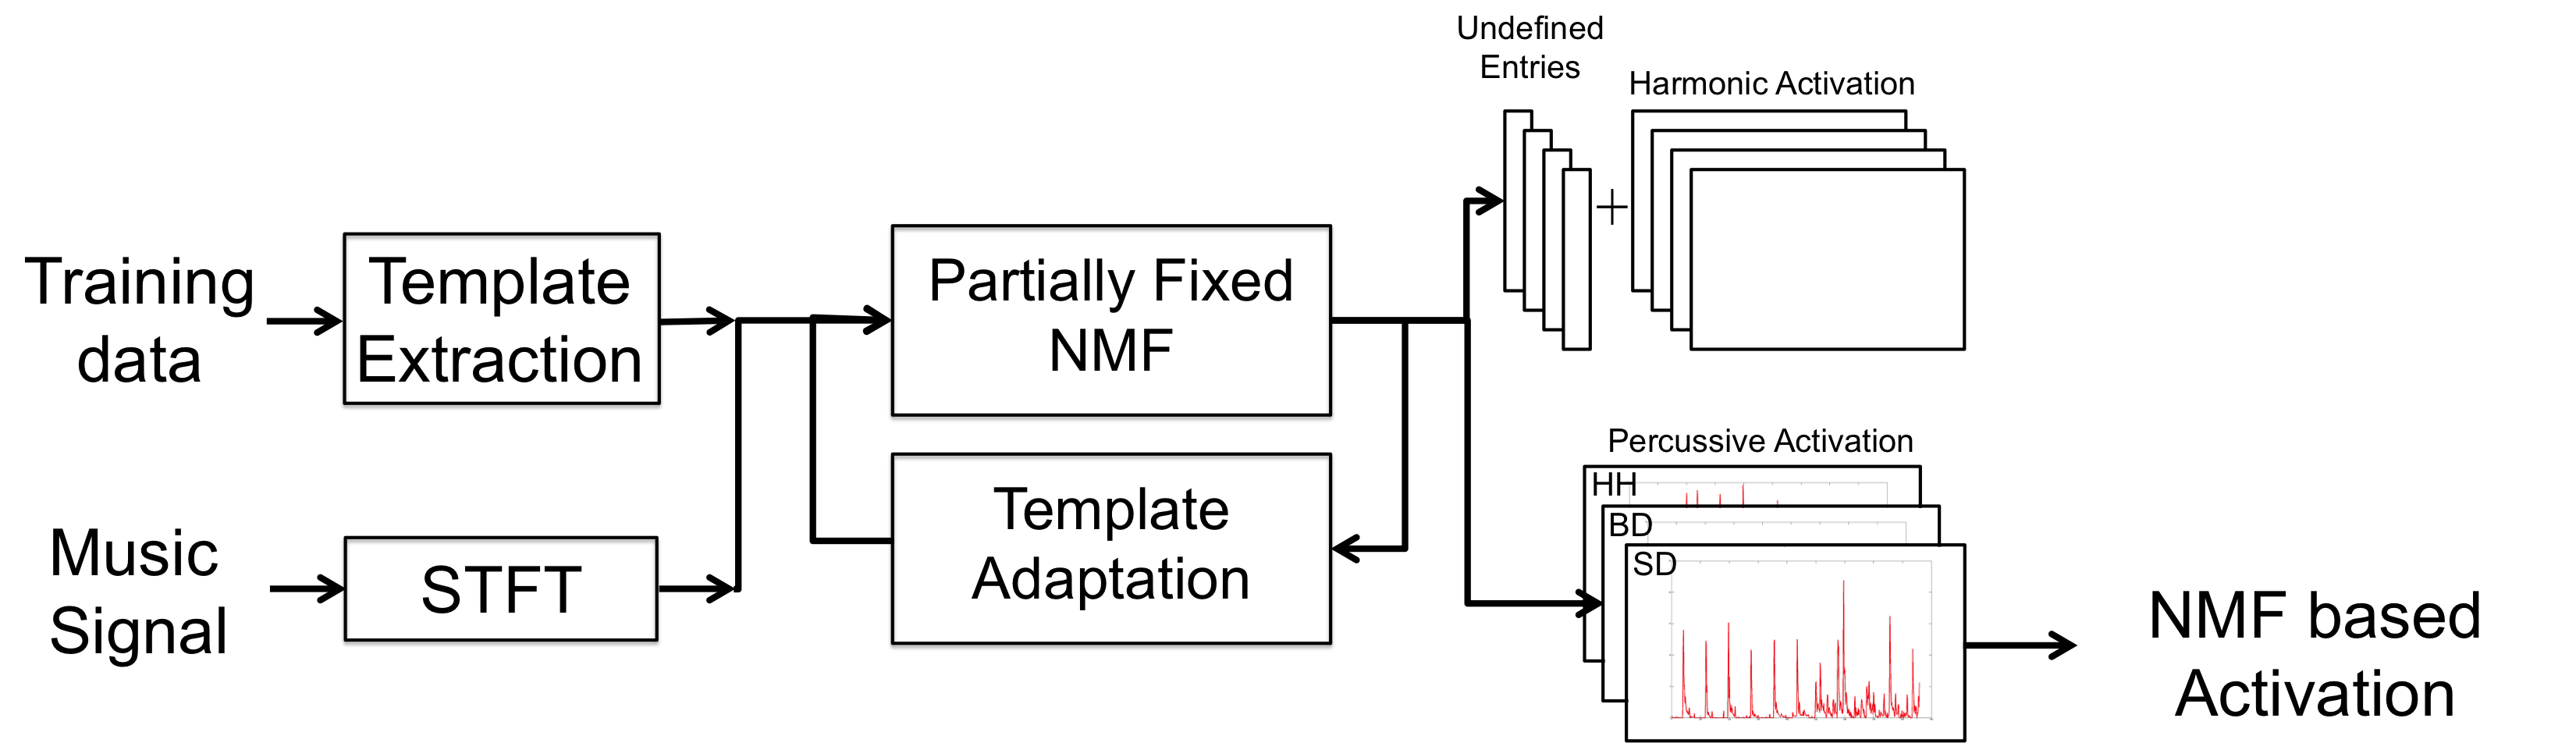
\includegraphics[width = 8.5 cm]{./figures/nmf.png}
\caption{Flowchart of the activation extraction process, see \cite{Wu2015a}}
\label{fig:nmf}
\end{figure}

\subsubsection{Activation Derived Features (ADF)}
\label{sssec:activ features}
Once the activation functions $h_{i}(n)$ have been extracted from the audio data, various features can be derived for further classification. The steps can be summarized as follows: first, for every given onset at index $n_{o}$, a \unit[400]{ms} segment centered around $h_{i}(n_{o})$ will be selected. Next, the maximum value of the segment will be positioned at the center. Then, we extract the distribution features, the Inter-Onset Interval (IOI) features, and the peak features from this segment as described below. 

\begin{enumerate}
	\item \textbf{Distribution features, $d = 5$}: Spread, Skew, Crest, Centroid, and Flatness. These features are similar to the commonly used spectral features, which provide the general description of the pattern. 
	\item \textbf{IOI features, $d = 2$}: IOI mean, and IOI standard deviation. These features are simple statistics of the IOI histogram.
	\item \textbf{Peak features, $d = 8$}: side peak to main peak ratio $\alpha_{i}$, and side peak to main peak signed block index difference $\Delta b_{i}$ $i = \{1, 2, 3, 4\}$. These features are designed to describe the details of the patterns. To compute the peak features, first we find the local maxima and sort them in descending order, then we calculate the ratio and index difference between the side peak and the main (largest) peak as features.
	\item \textbf{DTW features, $d = 4$}: the cumulative cost of a Dynamic Time Warping (DTW) distance between the current and the 4 template activation functions. To compute the DTW features, a median activation template of each playing technique is trained from the training data, and the cumulative cost of every DTW template for the given segment can be calculated. The examples of the extracted DTW templates for each technique are shown in Fig.~\ref{fig:atvall}.\\
\end{enumerate}

Finally, the resulting feature vector has a dimension $d = 19$.

%{\color{red}{I don't like this structure. I would combine the enumerate with the text, maybe do a paragraph per feature category. Also, make sure the description is understandable; you could also provide a simple graph if that helps.}} 
%The IOI features of the activation function are designed to capture the general temporal consistency{\color{red}{I don't know what temporal consistency is captured here, what is that anyway?}} of the pattern, 
%whereas the peak features are designed to describe the details of the pattern. To compute the peak features, first we find the local maxima and sort them in descending order, then we calculate the ratio and index difference between the side peak and the main (largest) peak as features. Since we are looking for specific patterns in the activation functions to identify the playing techniques, the cumulative cost of a Dynamic Time Warping (DTW) between the current and the template activation function is also extracted as feature. To compute the DTW features, a median activation template of each playing technique is trained from the training data, and the cumulative cost of every DTW template for the given segment can be calculated. The examples of the extracted DTW templates for each technique are shown in Fig.~\ref{fig:atvall}. Finally, the resulting feature vector has a dimension $d = 19$. The features are listed as follows: {\color{red}{reread the DTW description to see if it is understandble. not completely sure...}}



 %% I need new plots here 
\begin{figure}
\centering
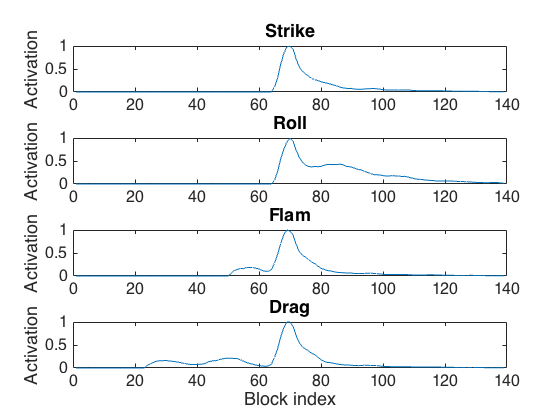
\includegraphics[width = 8 cm]{./figures/activ_all.png}
\caption{Examples of the extracted and normalized activation functions of (top to bottom): Strike, Buzz Roll, Flam, Drag}
\label{fig:atvall}
\end{figure}

\subsubsection{Timbre Features (TF)}
\label{sssec:timbre features}
To compare the effectiveness of the activation based features, a small set of the commonly used timbre features is extracted as well. The extraction process is similar to Sect.~\ref{sssec:activ features}, however, instead of using activation functions, the time-domain waveform of a given segment is used to derive the features. The features are: 

\begin{enumerate}
	\item \textbf{Spectral features, $d = 3$}: Centroid, Rolloff, Flux
	\item \textbf{Temporal features, $d = 1$}: Zero crossing rate
	\item \textbf{MFCCs, $d = 13$}: the first 13 MFCC coefficients
\end{enumerate}

The features are computed block by block using the same parameters as described in Sect.~\ref{sssec:activ}. The resulting feature vectors are further aggregated into one single vector by computing the mean and standard deviation of all the blocks. The final feature vector has a dimension $d = 34$. 

%\subsection{Classification}
%To compare and verify the effectiveness of the feature representations, two classifiers are tested in combinations with different feature sets. The first classifier is a multi-class C-SVM with Radial Basis Function (RBF) kernel and default parametrization. For the implementation, we used \textit{libsvm}\cite{Chang2011} in Matlab.  All of the features are scaled to a range between 0 and 1 using the standard min-max scaling approach before feeding into the SVM functions. 
%
%The second classifier is a feed-forward neural network with two hidden layers, each layer has 16 neurons. The output layer contains 4 neurons, and each neuron output indicates the likelihood of each playing technique being activated. For implementation, we used Matlab Neural Network Toolbox. 

\subsection{Dataset}
\subsubsection{Training Dataset}
\label{sssec:trainData}

% synthesis model example
\begin{figure} 
\centering
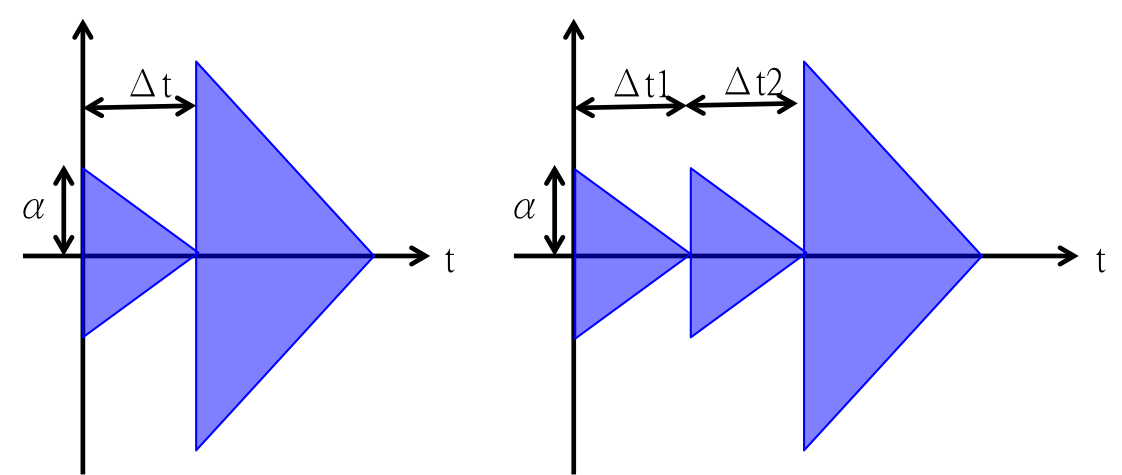
\includegraphics[width = 6.0 cm]{./figures/signal_model.png}
\caption{Illustration of the parametric forms of (Left) Flam and (Right) Drag}
\label{sigModel}
\end{figure}

In this paper, we focus on four different playing techniques (Strike, Flam, Drag, Buzz Roll) played on the snare drum. As can be seen in Table \ref{tab:data_all}, only Strike and Buzz Roll can be found in some of these datasets. Therefore, we generated a dataset through mixing existing recordings from MDLib 2.2 \cite{Prockup2013}. Since both Flam and Drag consist of preceding grace notes with different velocity and timing, they can be modeled with a limited set of parameters as shown in Fig.~\ref{sigModel}. The triangles in the figure represent the basic waveform excited by normal strikes, and the $\Delta t$ is the time difference between neighboring excitations. All the waveforms have been normalized to a maximum amplitude of -1 to 1, and the $\alpha$ is the amplitude ratio between the grace note and the strong note. 

In order to have realistic parameter settings for $\Delta t$ and $\alpha$, we annotated demo videos from Vic Firth's online lessons for both Flam\footnote{http://vicfirth.com/20-flam/ Last Access: 2016/03/16} and Drag.\footnote{http://vicfirth.com/31-drag/ Last Access: 2016/03/16} The final parameter settings and the details of the constructed dataset are shown in Table \ref{tab:our_data}. The parameters are based on the mean and standard deviation estimated from the videos. The resulting data contains all possible combinations of the parameters with the 144 mono snare Strike in the MDLib 2.2. However, to ensure the classifier is trained with uniformly distributed classes, only 576 randomly selected clips are used for Flam and Drag during the training. All of generated training data is available upon request.

\begin{table}[]
\footnotesize
\centering
\begin{tabular}{l|l|l}
\hline
\textbf{Techniques} & \textbf{Description} & \textbf{Total (\#clips)} \\ \hline
Strike & \begin{tabular}[c]{@{}l@{}}Snare excerpts from\\ MDLib 2.2 {[}16{]}\end{tabular} & 576 \\ \hline
Buzz Roll & \begin{tabular}[c]{@{}l@{}}Snare excerpts from\\ MDLib 2.2 {[}16{]}\end{tabular} & 576 \\ \hline
Flam & \begin{tabular}[c]{@{}l@{}}144 mono snare excerpts\\ $\alpha$ = \{0.1:0.1:0.7\}\\ $\Delta t$ = \{30:10:60\} (ms)\end{tabular} & 4032 \\ \hline
Drag & \begin{tabular}[c]{@{}l@{}}144 mono snare excerpts\\ $\alpha$ = \{0.15:0.1:0.55\}\\ $\Delta t_{1}$ = \{50:10:70\} (ms)\\ $\Delta t_{2}$ = \{45:10:75\} (ms)\end{tabular} & 8640 \\ \hline
\end{tabular}
\caption{An overview of the constructed dataset}
\label{tab:our_data}
\end{table}

\subsubsection{Test Dataset}
\label{ssec:testData}
To evaluate the system for detecting the playing techniques in polyphonic mixtures of music, the tracks from the ENST drum dataset minus one subset \cite{Gillet2006} have been annotated. The ENST drum dataset contains various drum recordings from 3 drummers with 3 different drum kits. The minus one subset, specifically, consists of 64 tracks of drum recordings with individual channel, mix, and accompaniments available. Since the playing technique is related to the playing style of the drummer, only 30 out of 64 tracks contain such techniques on snare drum. These techniques are annotated using the snare channel of the recordings, and each technique is labeled with the starting time, duration, and the technique index. As a result, a total number of 182 events (Roll: 109, Flam: 26, Drag: 47) have been annotated, and each event has a length of approximately 250 to 400 \unit{ms}. All of the above mentioned annotations are available online.\footnote{http://dummy link}

% briefly describe the dataset (3 drummers, 3 drum sets) individual channel as well as the mix
% minus one subset, 64 tracks with accompaniments
% provide: how did i annotate the data, (snare channel) number of events, durations
% the annotation are available dummy link

\section{Evaluation}\label{sec:eval}
\subsection{Metrics}\label{ssec:metrics}
For evaluating the accuracy on the testing data, we calculate the \textit{micro-averaged accuracy} and the \textit{macro-averaged accuracy}\cite{yang1999} to account for the unevenly distributed and sparse classes. The metrics are defined in the following equations:
\begin{equation}
micro~averaged = \frac{ \sum_{k = 1}^{K} C_{k} }{ \sum_{k = 1}^{K} N_{k} }
\end{equation}
\begin{equation}
macro~averaged = \frac{1}{K} \sum_{k = 1}^{K} (\frac{C_{k}}{N_{k}}),
\end{equation}
in which $K$ is the total number of classes, $N_{k}$ is the total number of samples in class $k$, and $C_{k}$ is the total number of correct samples in class $k$. These two metrics have different meanings: while each sample is weighted equally for the micro-averaged accuracy, the macro-averaged accuracy applies equal weight to each class, which gives a better overview of the performance by emphasizing the minority classes.
% mention it's very sparse
% we need micro and macro accuracy
% cite the first paper mentioning the micro and macro averaged accuracy

\subsection{Experiment Setup}
In this paper, three sets of experiments are conducted. The first experiment consists of running a 10-fold cross-validation on the training data, in the second experiment the test data is classified with an annotation-informed segmentation, and the third experiment classifies the test data without the annotation-informed segmentation. Different feature sets as described in Sect.~\ref{ssec:featuresExtract}, namely AF, ADF, and TF, are tested using a multi-class C-SVM with Radial Basis Function (RBF) kernel. For the implementation, we used \textit{libsvm}\cite{Chang2011} in Matlab.  All of the features are scaled to a range between 0 and 1 using the standard min-max scaling approach.
%{\color{red}{Earlier in this paragraph, I can also see a discussion or more detailed info, WHY Exp 1 and 2 make sense and why these 3 are chosen...}}

\subsection{Results}\label{ssec:results}
\begin{figure}
\centering
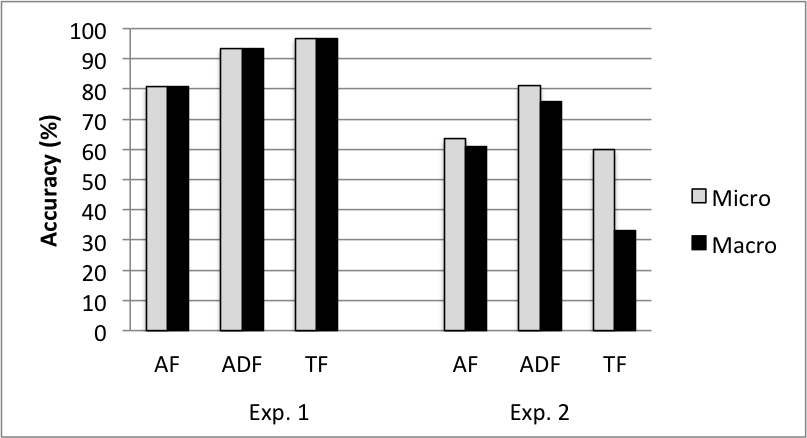
\includegraphics[width = 8.0 cm]{./figures/exp1_exp2.png}
\caption{Results of experiment 1 (left) and experiment 2 (right)}
\label{fig:exp1n2}
\end{figure}

\subsubsection{Experiment 1: Cross-Validation on Training Data}\label{sssec:exp1}
In Experiment 1, a 10-fold cross validation on the training data using different sets of features is performed. The results are shown in Fig.~\ref{fig:exp1n2} (left). This experimental setup is chosen for its similarity to the approaches described in previous work \cite{Tindale2004, Prockup2013}. As expected, the features allow to reliably separate the classes with accuracies between 80.9--96.8\% for the different feature sets. Since the training data contains 576 samples for all classes, the micro-averaged and marco-averaged accuracy are the same.
% each class has 576 samples

\subsubsection{Experiment 2: Annotation-Informed Testing}\label{sssec:exp2}
In Experiment 2, the same sets of features are extracted from the testing data for evaluation. Since the testing data is a completely different dataset with the real-world drum recordings, a verification of the feasibility of using the synthetic training data as well as the proposed feature representations is necessary. For this purpose, we simulate the best case scenario by using the snare channel as the input with an annotation-informed segmentation process. The resulting 182 segments are then classified using the trained SVM models from Experiment 1. With ADF, the best performance of 76.0 and 81.3\% was achieved for both macro and micro-averaged accuracy, respectively. This experiment serves as a sanity check to the presented scheme, and the results shown in Fig.~\ref{fig:exp1n2} (right) represent a glass ceiling for our experiment 3.
% we use the ground truth from the annotations to perfectly segment the playing technique events from the snare channel
% this is a proof of concept to see whether the pre-trained model actually works
% only consider a 3-class problem

\subsubsection{Experiment 3: Real-World Testing}\label{sssec:exp3}
\begin{figure}
\centering
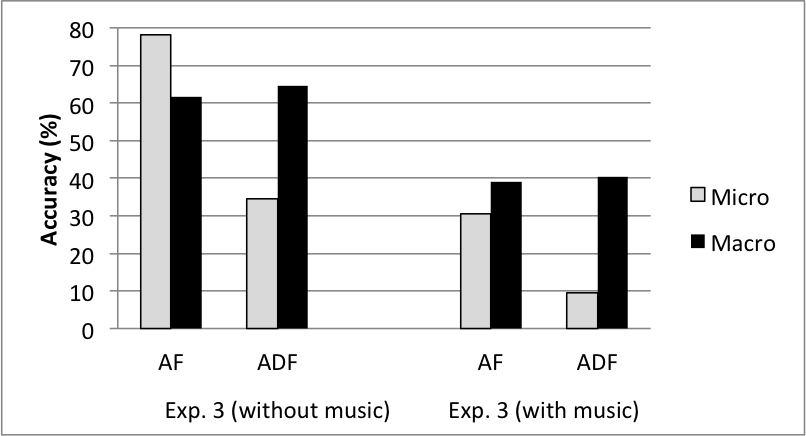
\includegraphics[width = 8.0 cm]{./figures/exp3.png}
\caption{Results of experiment 3 without background music (left) and with background music (right)}
\label{fig:exp3}
\end{figure}
Experiment 3 utilizes a more realistic setup and is our main experiment. Each onset is examined and classified without any prior knowledge about the segmentation. A fixed region around each onset is segmented and classified. As a result, a total number of 2943 onsets (including the previous mentioned 182 playing technique events and 2761 strikes) are evaluated. Since the timbre features do not show promising results in Experiment 2, they are excluded from this experiment. To investigate the influence of the background music, both the recordings of the snare channel and the complete polyphonic mixtures are tested. The results are shown in Fig.~\ref{fig:exp3}. Without the background music, the best macro-averaged accuracy is 64.6\% using ADF, and the best micro-averaged accuracy is 78.0\% using AF. With the background music, the best macro-averaged accuracy is 40.4\% using ADF, and the best micro-averaged accuracy is 30.4\% using AF. 

% real-world scenario where the duration of the playing technique is unknown
% use a fixed window
% now it's a 4-class problem
% first, without accompaniments 
% results show that when the signal is clean, this method is able to detect the playing techniques on the real-world performances

% with music
% everything dropped 
% still a way to go
\subsection{Discussion}
\label{ssec:discussion}
Based on the experiment results, the following observations can be made: 

% good: timbre feature vs activation features
First,  as can be seen in Fig.~\ref{fig:exp1n2}, the timbre features achieve the highest cross-validation accuracy in Experiment 1, which shows their effectiveness in differentiating our classes. This observation echos the results from the related work, which demonstrate the usefulness of timbre features for distinguishing the different sounds. However, when these features are applied to classify a completely different dataset, they are unable to recognize the same pattern played with different drum sounds. As a result, the timbre features achieve the lowest macro-averaged accuracy in Experiment 2, and the micro-averaged accuracy approximates the Zero-R accuracy by always predicting the majority class. 
This result shows that timbre features might not be directly applicable to detecting the playing techniques in unknown recordings. The activation functions and activation derived features, on the other hand, are relatively stable and consistent between the micro and macro-averaged accuracy. This indicates a better performance for detecting the proposed playing techniques in the unseen dataset. 

% good: activation vs activation features
Second, in comparison with the raw activation functions, the activation-derived features tend to achieve a higher macro-averaged accuracy than the activation functions among all experiment results. Furthermore, the activation-derived features are more sensitive to different playing techniques, whereas the activation functions are more sensitive to strikes. 
These results indicate that the activation derived features are more capable of detecting the playing techniques. This tendency can also be seen in the confusion matrices in Tables~\ref{EXP3_music_AF} and \ref{EXP3_music_ADF}, where the activation derived features perform better than the activation functions in Roll and Drag, and slightly worse in Flam. The activation functions generally achieve higher micro-averaged accuracy than the activation-derived features. Since the distribution of the classes is skewed towards Strike in the testing data, the micro-averaged accuracy of the activation functions is largely increased by a higher rate of detecting strikes.

\begin{table}[]
\centering
\begin{tabular}{l|llll}
       & Strike & Roll & Flam & Drag \\ \hline
Strike (2761) & 28.9   & 38.8 & 5.7  & 26.6 \\
Roll (109)  & 8.3    & 66.1 & 11.9 & 13.8 \\
Flam (26)  & 3.8    & 53.8 & 19.2 & 23.1 \\
Drag (47)  & 46.8   & 6.4  & 4.3  & 42.6
\end{tabular}
\caption{Confusion matrix of Exp.~3 with music and AF (in \%)}
\label{EXP3_music_AF}
\end{table}

\begin{table}[]
\centering
\begin{tabular}{l|llll}
      & Strike & Roll & Flam & Drag \\ \hline
Strike (2761) & 5.8    & 62.9 & 3.8  & 27.6 \\
Roll (109)  & 5.5    & 74.3 & 3.7  & 16.5 \\
Flam (26)  & 0.0    & 61.5 & 11.5 & 26.9 \\
Drag (47)  & 2.1    & 8.5  & 19.1 & 70.2
\end{tabular}
\caption{Confusion matrix of Exp.~3 with music and ADF (in \%)}
\label{EXP3_music_ADF}
\end{table}

% neural: in polyphonic mixtures, what techniques are easily confused with each other?
Third, according to the confusion matrices (Tables~ \ref{EXP3_music_AF} and \ref{EXP3_music_ADF}), Strike and Flam can be easily confused with Roll for both features in the context of polyphonic mixtures of music. One possible explanation is that, whenever the signal is not properly segmented, the activation function will contain overlapping activities from the previous or the next onset, which might result leakage to the original activation and make it resemble a Roll. The strong skewness towards the preceding grace notes in the case of Drag makes it relatively easy to distinguish from Roll for both features.  

% bad: poor results in the polyphonic mixtures
Fourth, for both activation functions and activation derived features, the detection performance drops drastically in Experiment 3 with the presence of background music. The reason could be that with the background music, the extracted activation function becomes noisier due to the imperfect decomposition. Since the classification models are trained on the clean signals, they might be susceptible to these disturbance. As a result, the classifier might be tricked into classifying Strike as other playing techniques, decreasing the micro-averaged accuracy. 

% bad: finally, we bypass the onset detection problem here. In the real-world scenario, the error might propagate.
%{\color{red}{I am not sure about this. The location is definitely weird. Leave it out?}}
Additionally, the proposed method does not take into account the onset detection at this moment. By adding the onset detection process to the loop, the detection accuracy could be further reduced, which increases the difficulty of direct application of the method in the polyphonic mixtures. 

%{\color{red}{The following sentence is conclusion, not discussion}}To build a system towards retrieving the playing techniques reliably from the polyphonic mixtures of music, further improvements are necessary.  

\section{Conclusion}
\label{sec:conclusion}
In this paper, a system working towards drum playing technique detection in the polyphonic mixtures of music has been presented. To achieve this goal, two datasets have been generated for training and testing purposes. The experiment results indicate that the current method is able to detect the playing techniques from the real-world drum recordings when the signal is relatively clean. However, low accuracy of the system in the presence of background music indicates that more sophisticated approaches should be applied in order to improve the detection of playing techniques in polyphonic mixtures of music. 

The possible directions for the future work are: first, investigate different source separation algorithms as a pre-processing step in order to get a cleaner representation. The results of Experiments 2 and 3 show that a cleaner input representation improves both the micro and macro-averaged accuracy by more than 20\%. Therefore, a good source separation method to isolate the snare drum sound could be beneficial. Common techniques such as HPSS and and other approaches for source separation should be investigated.

Second, since the results in Experiment 3 implies that the system is susceptible to the disturbance from background music, a classification model trained on the slightly noisier data could possibly increase the robustness against the presence of unwanted sounds. The influence of adding different levels of random noise while training could be evaluated.

Third, the current dataset offers only a limited number of samples for the evaluation of playing technique detection in polyphonic mixtures of music. Due to the sparse nature of these playing techniques, their occurrence in existing datasets is rare and difficult to collect and annotate. However, to arrive at a statistically more meaningful conclusion, additional  data would be necessary.

Last but not least, different state-of-the-art classification methods, such as deep neural networks, could also be applied to this task in searching for a better solution.

% the real-world case is okay... maybe preprocessing or source separation will help 

% 4. although the accuracy of the current system in the polyphonic mixtures is still low, it demonstrates the potential of using activation-based features
%     for transcribing subtle gestures from the audio signals.
% 5. future work: pre-processing steps for source separation, better segmentation schemes, and test other classifiers



% For bibtex users:
\bibliography{cw_ismir2016}

% For non bibtex users:
%\begin{thebibliography}{citations}
%
%\bibitem {Author:00}
%E. Author.
%``The Title of the Conference Paper,''
%{\it Proceedings of the International Symposium
%on Music Information Retrieval}, pp.~000--111, 2000.
%
%\bibitem{Someone:10}
%A. Someone, B. Someone, and C. Someone.
%``The Title of the Journal Paper,''
%{\it Journal of New Music Research},
%Vol.~A, No.~B, pp.~111--222, 2010.
%
%\bibitem{Someone:04} X. Someone and Y. Someone. {\it Title of the Book},
%    Editorial Acme, Porto, 2012.
%
%\end{thebibliography}

\end{document}
